% Constructed and checked from the problem; not a geometric proof.
\documentclass[tikz,border=8pt]{standalone}
\begin{document}
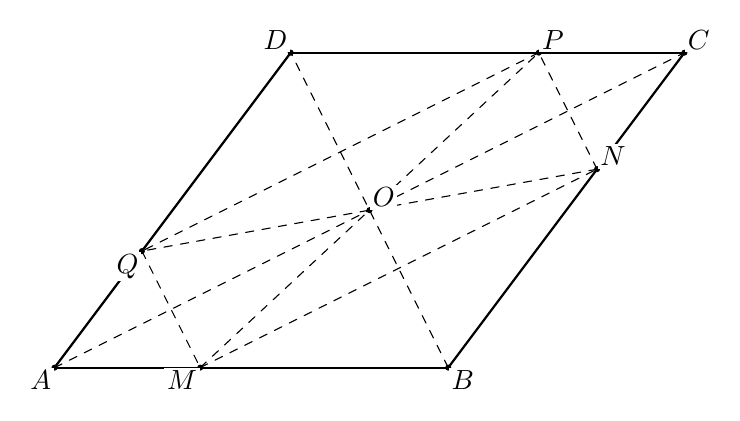
\begin{tikzpicture}[scale=1,line cap=round,line join=round]
\coordinate (p0) at (0,0);
\coordinate (p1) at (5,0);
\coordinate (p2) at (8,4);
\coordinate (p3) at (3,4);
\coordinate (p4) at (4,2);
\coordinate (p5) at (1.85,0);
\coordinate (p6) at (6.89,2.52);
\coordinate (p7) at (6.15,4);
\coordinate (p8) at (1.11,1.48);
\draw[thick] (p0) -- (p1);
\draw[thick] (p1) -- (p2);
\draw[thick] (p2) -- (p3);
\draw[thick] (p3) -- (p0);
\draw[dashed] (p0) -- (p2);
\draw[dashed] (p1) -- (p3);
\draw[dashed] (p5) -- (p6);
\draw[dashed] (p6) -- (p7);
\draw[dashed] (p7) -- (p8);
\draw[dashed] (p8) -- (p5);
\draw[dashed] (p5) -- (p7);
\draw[dashed] (p6) -- (p8);
\fill (p0) circle (1.1pt) node[fill=white,inner sep=1pt,below left] {$A$};
\fill (p1) circle (1.1pt) node[fill=white,inner sep=1pt,below right] {$B$};
\fill (p2) circle (1.1pt) node[fill=white,inner sep=1pt,above right] {$C$};
\fill (p3) circle (1.1pt) node[fill=white,inner sep=1pt,above left] {$D$};
\fill (p4) circle (1.1pt) node[fill=white,inner sep=1pt,above right] {$O$};
\fill (p5) circle (1.1pt) node[fill=white,inner sep=1pt,below left] {$M$};
\fill (p6) circle (1.1pt) node[fill=white,inner sep=1pt,above right] {$N$};
\fill (p7) circle (1.1pt) node[fill=white,inner sep=1pt,above right] {$P$};
\fill (p8) circle (1.1pt) node[fill=white,inner sep=1pt,below left] {$Q$};
\end{tikzpicture}
\end{document}
